\newpage
\section{METHODOLOGY}
Image Super Resolution is a branch of Artificial Intelligence that deals with
upscaling a Low-Resolution Image to High Resolution Image, filling in the missing
pixels with the help of learning from the environment using machine learning. There
are other methods of upscale images like Linear or Bi-cubic interpolation but they do
not generate any new information based on the environment and hence are not super
useful to upscale an LR image. The retrieval of High-Resolution images based on
underlying image is not new, there were techniques such as sparse representation-based
methods. However, it was the advent of deep learning and convolutional neural
networks that arguably brought about the most significant leaps forward, with the
seminal work being the Super-Resolution Convolutional Neural Network (SRCNN)
proposed by Dong et al. in 2014. Much work has been done since then, not only on the
design and structure of the neural networks but also on the data used to train and
evaluate these networks. Deep Learning based methods require huge amounts of data
so that the model is not overfitted, the dataset needs to contain an HR and LR version of
the same image. Images must be perfectly aligned to each other. To do so, the LR image
is obtained by synthetically degrading image using a degradation model. 

The ‘classical’ degradation model is the most commonly used, which considers
down-sampling, blurring, and noise: 
$$I^{LR}= (I^{HR} \circledast k)\downarrow_s + n$$
where $\circledast$ represents a convolution operation, k is a kernel (typically a Gaussian blurring
kernel, but it can also represent other functions such as the Point Spread Function
(PSF)), n represents additive noise, and ↓s is a downscaling operation that is typically
assumed to be bicubic down-sampling with scale factor s.
The aim of SR is to then reverse whichever degradation process is considered, to
retrieve the original underlying high-fidelity image. Some of popular methods to
perform this task are: 
\subsection{Non-Blind SR Methods}
\begin{enumerate}
    \item {\bf SRCNN:}The Super-Resolution Convolutional Neural Network (SRCNN) is considered to be the
    pioneering work in using deep learning and convolutional neural networks for the task of SR. It only consists of three layers and requires the LR image to be up-sampled using
    bicubic interpolation prior to being processed by the network, but it was shown to outperform the state-of-the-art methods of the time such as A+ and the sparse representation-based method. It was also shown that sparse-coding-based methods are equivalent to convolutional neural networks, which influenced SRCNN’s hyperparameter settings. While SRCNN has been used as a benchmark by numerous researchers, it is now comprehensively outclassed and is no longer used so frequently.
    \begin{figure}[ht]
        \centering
        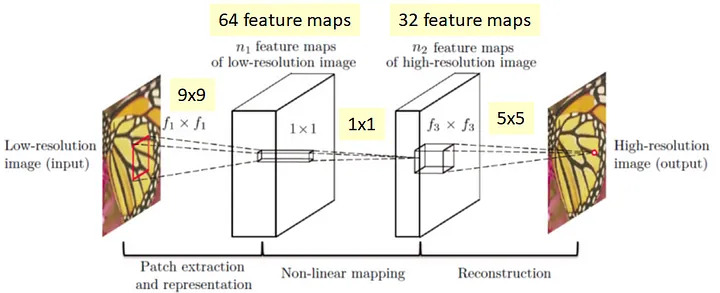
\includegraphics[width=5in]{./figures/srcnn.jpg}
        \caption{SRCNN Representation}
    \end{figure}
\end{enumerate}